\documentclass[conference]{IEEEtran}
\usepackage[utf8]{inputenc}
\usepackage[T1]{fontenc}
\usepackage[turkish]{babel}
\usepackage{graphicx}
\usepackage{float}
\usepackage{caption}
\usepackage{listings}
\usepackage{algorithm}
\usepackage{algpseudocode}
\usepackage{xurl}
\usepackage{placeins}
\usepackage{array}
\usepackage{dblfloatfix}
\usepackage[hidelinks]{hyperref}

\graphicspath{{figures/}{report/figures/}}

\newcommand{\LongState}[1]{%
	\State \parbox[t]{\dimexpr\linewidth-\algorithmicindent\relax}{#1}%
}

\setkeys{Gin}{width=0.92\columnwidth,keepaspectratio}

\makeatletter
\renewenvironment{abstract}{%
	\par\noindent
	{\normalfont\normalsize ÖZET}\par\medskip
	\normalfont\normalsize
}{%
	\par
}
\makeatother

\title{%
	\normalsize\bfseries
	KOCAELİ ÜNİVERSİTESİ BİLGİSAYAR MÜHENDİSLİĞİ\\[1em]
	YAZILIM LABORATUVARI - II\\
	PROJE - III\\[1em]
	Araba Gövde Tipi Sınıflandırma Projesi
}

\author{
	\IEEEauthorblockN{Saffet Hakan KOÇAK}
	\IEEEauthorblockA{%
		Bilgisayar Mühendisliği\\
		Kocaeli Üniversitesi\\
		230202058%
	}
	\and
	\IEEEauthorblockN{Yusuf BÜLBÜL}
	\IEEEauthorblockA{%
		Bilgisayar Mühendisliği\\
		Kocaeli Üniversitesi\\
		230202050%
	}
}

\begin{document}
\maketitle

\begin{abstract}
Bu projede, sekiz farklı araba gövde tipini görüntüler üzerinden
sınıflandıran derin öğrenme tabanlı bir sistem geliştirilmiştir. Çalışmada
SUV, VAN, STATION\_WAGON, MICRO, OPEN\_WHEEL, SEDAN, HATCHBACK ve PICK\_UP
sınıfları kullanılmış; farklı açık kaynak veri kümeleri ve manuel seçilen
görseller birleştirilerek özelleştirilmiş bir veri seti oluşturulmuştur.
Veri seti, eğitim sürecinde sınıf dengesini koruyacak şekilde
hazırlanmış ve modelin daha önce görmediği test verileri üzerindeki
genelleme başarısı ölçülmüştür.
\vspace{0.4cm}

Model mimarisi olarak, dosya boyutu ve hız kısıtları dikkate alınarak
EfficientNet-B2 seçilmiştir. EfficientNet-B0, EfficientNet-B1, ResNet18 ve
EfficientNet-B3 gibi alternatifler denenmiş; başarı, macro F1, model boyutu
ve çalışma verimliliği birlikte değerlendirilmiştir. Final model, ImageNet
üzerinde önceden eğitilmiş ağırlıklar ile başlatılmış, son sınıflandırıcı
katmanı sekiz sınıfa uygun hale getirilmiş ve Google Colab ortamında
eğitilmiştir. Final modelde görüntü oranını bozmamak için
ResizeWithPadding(224), tensor dönüşümü ve ImageNet normalizasyonu
kullanılmıştır.
\vspace{0.4cm}

Elde edilen model, test veri setinde 0.9698 doğruluk ve 0.9700 macro
F1-skoru üretmiştir. Sonuçlar; sınıf bazlı precision, recall ve F1
değerleri, eğitim/doğrulama loss ve accuracy grafikleri, validation macro
F1 eğrisi ve normalize edilmiş karışıklık matrisi ile analiz edilmiştir.
Model, ayrıca Streamlit tabanlı bir web arayüzüne entegre edilerek tek
görsel üzerinde canlı tahmin yapabilir hale getirilmiştir.
\vspace{0.4cm}

Hocaların nihai test sürecinde kullanacağı formata uyum sağlamak amacıyla
ayrı bir PredictionScript.txt dosyası hazırlanmıştır. Bu script,
testdata klasörünü recursive olarak gezmekte, modeli yüklemekte ve her
görsel için ``filename.jpg | Pred: class\_id'' biçiminde Preds.txt çıktısı
üretmektedir. Böylece geliştirilen model hem proje arayüzünde hem de
otomatik değerlendirme ortamında kullanılabilir hale getirilmiştir.
\vspace{0.4cm}
\end{abstract}

\section{GİRİŞ}

Görüntü tabanlı araç sınıflandırma problemleri, trafik izleme, otopark
yönetimi, sigorta süreçleri, ikinci el araç analizi ve akıllı ulaşım
sistemleri gibi pek çok uygulama alanında kullanılmaktadır. Araçların marka
ve modelinden bağımsız olarak gövde tiplerinin tanınması ise daha genel ve
pratik bir sınıflandırma problemi sunar. Bu çalışmada amaç, farklı araba
gövde tiplerini sekiz sınıfa ayırabilen, düşük boyutlu ve açıklanabilir bir
derin öğrenme sistemi geliştirmektir.
\vspace{0.4cm}

Proje kapsamında SUV, VAN, STATION\_WAGON, MICRO, OPEN\_WHEEL, SEDAN,
HATCHBACK ve PICK\_UP sınıfları ele alınmıştır. Bu sınıflar bazı durumlarda
birbirine görsel olarak oldukça yakındır. Özellikle SEDAN-HATCHBACK,
SUV-HATCHBACK ve STATION\_WAGON-SEDAN ayrımları, aracın arka çıkıntısı,
tavan çizgisi, yerden yüksekliği ve bagaj formu gibi ayırt edici görsel
özelliklere bağlıdır. Bu nedenle veri setinin temizliği, sınıf dengesi ve
preprocessing seçimi model başarısı açısından kritik hale gelmiştir.
\vspace{0.4cm}

Raporun devamında veri toplama ve hazırlama süreci, kullanılan
preprocessing adımları, EfficientNet-B2 mimarisi, eğitim ayarları,
değerlendirme sonuçları, web arayüzü ve teslim entegrasyonu ayrıntılı
biçimde açıklanmaktadır.

\section{YÖNTEM}

\subsection{Veri Seti Oluşturma}

Veri seti, Kaggle üzerinde bulunan Cars Body Type Cropped ve Stanford Car
Body Type Data veri kümelerinden yararlanılarak oluşturulmuştur. Bu veri
kümelerinde proje sınıflarıyla doğrudan uyuşan klasörler uygun sınıflara
aktarılmış; sınıf uyuşmazlığı olan Convertible, Coupe, Cab, Minivan ve
Other gibi kategoriler yanlış etiket riskinden dolayı kullanılmamıştır.
\vspace{0.4cm}

MICRO, OPEN\_WHEEL, STATION\_WAGON, SUV, SEDAN, HATCHBACK ve PICK\_UP
sınıflarında eksik veya kalite açısından zayıf kalan görseller için ek
aday görsel toplama scriptleri hazırlanmıştır. Bu scriptlerde DuckDuckGo
görsel arama sonuçları kullanılmış, indirilen görseller önce aday
klasörlerinde toplanmış ve manuel kontrol sonrasında yalnızca uygun
görseller seçilmiştir. Böylece modelin yanlış etiketli veya alakasız
görsellerle eğitilmesi azaltılmıştır.
\vspace{0.4cm}

Ham veri seti \texttt{dataset/raw} altında tutulmuş, eğitim için kullanılan
son veri seti ise \texttt{dataset/processed} klasörüne kopyalama yöntemiyle
hazırlanmıştır. Ham veri setine zarar vermemek için split işlemi raw
klasörünü değiştirmemektedir. Desteklenen görsel uzantıları .jpg, .jpeg,
.png, .bmp ve .webp olarak belirlenmiştir.
\vspace{0.4cm}

Veri hazırlama sürecinde yalnızca görsel sayısını artırmak değil, etiket
kalitesini korumak da temel hedeflerden biri olmuştur. Bu nedenle özellikle
SEDAN, HATCHBACK ve STATION\_WAGON gibi birbirine yakın gövde tiplerinde
aday görseller manuel olarak kontrol edilmiştir. Yan açıdan çekilmeyen,
aracın büyük kısmı görünmeyen, farklı araç türleri içeren veya sınıf
tanımına uymayan örnekler veri setinden çıkarılmıştır. Böylece modelin
sınıf ayrımını yanlış etiketlerden öğrenmesi azaltılmaya çalışılmıştır.

\subsection{Sınıf Dağılımı}

Her sınıftan en fazla 1000 geçerli görsel kullanılacak şekilde dengeli
veri seti hazırlanmıştır. MICRO sınıfında 1000'den az görsel bulunduğu
için bu sınıftaki tüm geçerli görseller kullanılmıştır. Seçilen görseller
sınıf bazlı olarak yaklaşık yüzde 80 eğitim, yüzde 10 doğrulama ve yüzde
10 test olacak biçimde ayrılmıştır. Split işlemi seed=42 ile deterministik
hale getirilmiştir.

\begin{table}[H]
\centering
\caption{Veri Seti Dağılımı}
\label{tab:dataset_distribution}
\small
\begin{tabular}{|l|r|r|r|r|}
\hline
\textbf{Sınıf} & \textbf{Raw} & \textbf{Train} & \textbf{Val} & \textbf{Test} \\
\hline
SUV & 2703 & 800 & 100 & 100 \\
VAN & 1215 & 800 & 100 & 100 \\
STATION\_WAGON & 1015 & 800 & 100 & 100 \\
MICRO & 952 & 761 & 95 & 96 \\
OPEN\_WHEEL & 1221 & 800 & 100 & 100 \\
SEDAN & 2914 & 800 & 100 & 100 \\
HATCHBACK & 1589 & 800 & 100 & 100 \\
PICK\_UP & 1114 & 800 & 100 & 100 \\
\hline
\textbf{Toplam} & \textbf{12723} & \textbf{6361} & \textbf{795} & \textbf{796} \\
\hline
\end{tabular}
\end{table}

\FloatBarrier
\begin{figure}[htbp]
	\centering
	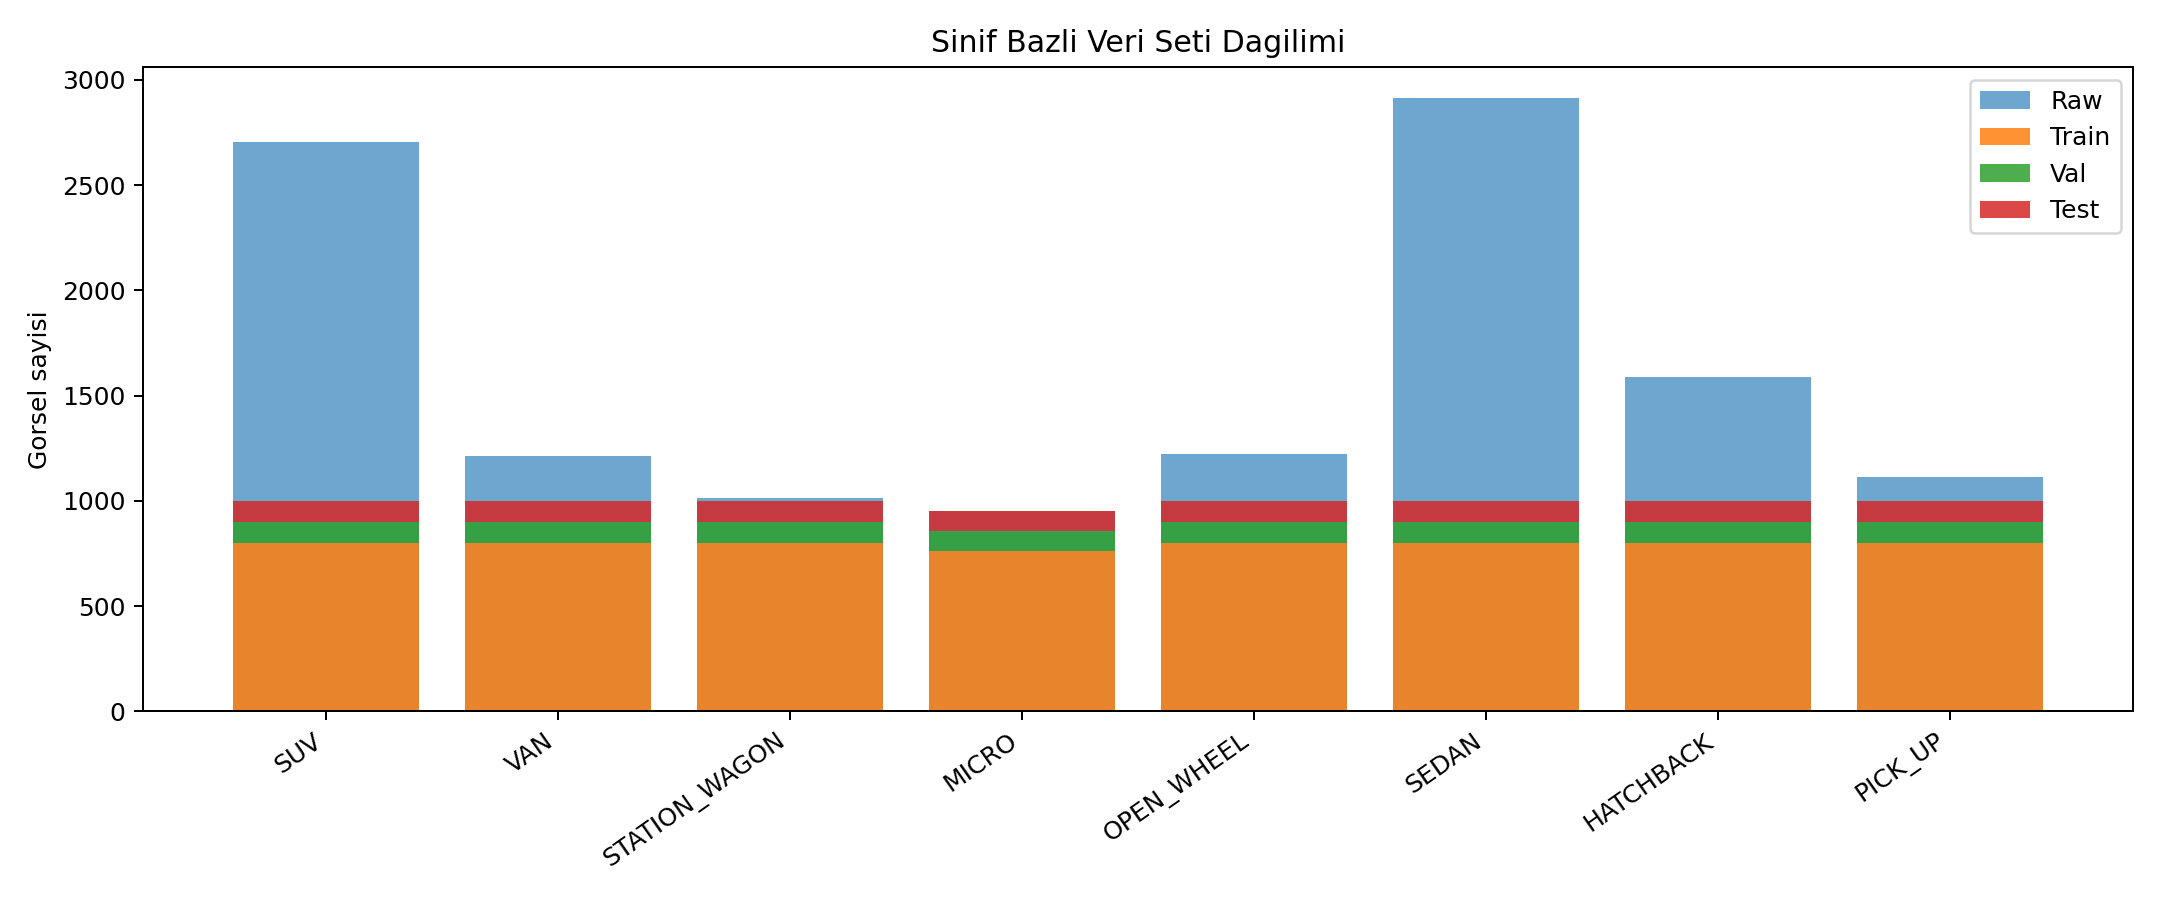
\includegraphics{dataset_distribution.png}
	\caption{Sınıf bazlı ham ve işlenmiş veri dağılımı}
	\label{fig:dataset_distribution}
\end{figure}

\subsection{Ön İşleme ve Veri Artırma}

Final model B2 V4 olarak adlandırılmıştır. Bu modelde görüntünün en-boy
oranının bozulmaması için doğrudan 224x224 boyutuna sıkıştırma yerine
padding tabanlı yeniden boyutlandırma kullanılmıştır. ResizeWithPadding
adımı önce görüntüyü 224x224 alanına sığacak şekilde küçültür veya
büyütür, ardından boş kalan alanları siyah arka plan ile tamamlar. Böylece
araçların yatay/dikey oranı korunur.
\vspace{0.4cm}

Eğitim tarafında veri artırma için yatay çevirme, küçük açılı döndürme ve
hafif renk değişimleri kullanılmıştır. Doğrulama, test ve tahmin
tarafında ise aynı sabit preprocessing uygulanmıştır: ResizeWithPadding(224),
ToTensor ve ImageNet mean/std ile normalizasyon.
\vspace{0.4cm}

Preprocessing adımlarının tüm eğitim dışı kullanım noktalarında aynı
tutulması özellikle önemlidir. Çünkü model, eğitim sırasında belirli bir
görüntü ölçekleme ve normalizasyon dağılımına göre öğrenmektedir. Web
arayüzü, test değerlendirme kodu ve PredictionScript dosyasında aynı
ResizeWithPadding(224) ve aynı ImageNet normalizasyon değerleri
kullanılarak eğitim-tahmin dağılım farkı azaltılmıştır.

\subsection{Model Adayları ve Seçim Süreci}

Proje sırasında tek bir modelle ilerlemek yerine farklı CNN mimarileri
karşılaştırılmıştır. Karşılaştırmada yalnızca accuracy değerine değil,
sınıflar arası dengeyi daha iyi gösterdiği için macro F1 değerine de
dikkat edilmiştir. Ayrıca proje tesliminde model dosyası için 95 MB sınırı
bulunduğundan, model boyutu ve tahmin hızı da seçim kriterleri arasında
değerlendirilmiştir.

\begin{table}[H]
\centering
\caption{Denenen Model Adaylarının Karşılaştırılması}
\label{tab:model_comparison}
\scriptsize
\resizebox{\columnwidth}{!}{%
\begin{tabular}{|l|r|r|r|r|l|}
\hline
\textbf{Model} & \textbf{Accuracy} & \textbf{Macro Precision} & \textbf{Macro Recall} & \textbf{Macro F1} & \textbf{Durum} \\
\hline
EfficientNet-B0 & 0.9523 & 0.9528 & 0.9523 & 0.9523 & Elendi \\
EfficientNet-B1 & 0.9661 & 0.9662 & 0.9662 & 0.9661 & İyi \\
ResNet18 & 0.9686 & 0.9697 & 0.9687 & 0.9688 & Çok iyi \\
\textbf{EfficientNet-B2} & \textbf{0.9698} & \textbf{0.9710} & \textbf{0.9699} & \textbf{0.9700} & \textbf{Final model} \\
EfficientNet-B3 & 0.9636 & 0.9646 & 0.9636 & 0.9638 & B2 modelinden düşük \\
\hline
\end{tabular}%
}
\end{table}

EfficientNet-B0 modeli küçük ve hızlı olmasına rağmen sınıflar arası
ayrımda B1, B2 ve ResNet18 kadar güçlü sonuç üretmemiştir. EfficientNet-B1
başarılı bir ara seçenek olmuştur; ancak final test sonuçlarında B2'nin
gerisinde kalmıştır. ResNet18 modeli beklenenden güçlü sonuç vermiş, fakat
EfficientNet-B2 hem macro F1 hem de genel başarı açısından daha dengeli
bir sonuç sunduğu için final aday olarak öne çıkmıştır.
\vspace{0.4cm}

EfficientNet-B3 daha büyük bir model olmasına rağmen bu veri setinde B2'den
daha yüksek başarı üretmemiştir. Bu durum daha büyük modelin her zaman daha
iyi genelleme yapmadığını göstermektedir. Veri seti boyutu, sınıflar arası
benzerlikler ve model karmaşıklığı birlikte değerlendirildiğinde
EfficientNet-B2, başarı, dosya boyutu ve çalışma hızı açısından en uygun
dengeyi sağlamıştır. Tablo \ref{tab:model_comparison}'daki EfficientNet-B2
satırı, teslimde kullanılan final modelin mevcut test sonuçlarını
göstermektedir.

\subsection{Model Mimarisi}

Final model olarak EfficientNet-B2 kullanılmıştır. EfficientNet ailesi,
genişlik, derinlik ve çözünürlük ölçeklemelerini dengeli biçimde kullanan
verimli CNN mimarilerinden biridir. Bu mimaride model kapasitesi yalnızca
katman sayısı artırılarak değil, ağ genişliği ve giriş çözünürlüğü ile
birlikte dengeli şekilde ölçeklenmektedir. Bu nedenle EfficientNet
modelleri, benzer başarı düzeylerinde daha kompakt dosya boyutu ve daha
verimli çalışma süresi sunabilmektedir.
\vspace{0.4cm}

Bu proje için EfficientNet-B2'nin seçilmesinin temel nedeni, B0 ve B1'e göre
daha yüksek ayırt edici kapasiteye sahip olması, B3'e göre ise daha kararlı
ve daha küçük bir final model üretmesidir. Ayrıca ResNet18'e çok yakın veya
daha iyi sonuçlar verirken modern ve parametre açısından verimli bir mimari
sunmuştur. Böylece model, hem web arayüzünde canlı tahmin için yeterince
hızlı kalmış hem de teslim sınırı olan 95 MB model boyutunun oldukça altında
29.86 MB'lık bir \texttt{state\_dict} dosyası ile kullanılabilir hale
gelmiştir.
\vspace{0.4cm}

Model torchvision kütüphanesindeki EfficientNet-B2 mimarisi üzerinden
kurulmuştur. ImageNet ön eğitimli ağırlıklar kullanılmış ve son
sınıflandırıcı katman sekiz sınıfa göre değiştirilmiştir. Final Colab
eğitiminde sınıflandırıcı katmanda Dropout(p=0.4) ve Linear(in\_features, 8)
yapısı kullanılmıştır. ImageNet ön eğitimli ağırlıklar sayesinde model,
kenar, doku, parça ve genel nesne formu gibi düşük ve orta seviye görsel
özellikleri hazır bir başlangıç noktasından öğrenmeye başlamıştır. Son
katman sekiz gövde tipine göre yeniden düzenlenmiş ve model bu veri seti
üzerinde ince ayar yöntemiyle eğitilmiştir. Model kaydedilirken yalnızca
\texttt{state\_dict} kaydedilmiş, optimizer veya eğitim geçmişi model
dosyasına dahil edilmemiştir.

\begin{table}[H]
\centering
\caption{Final Model ve Eğitim Ayarları}
\label{tab:model_settings}
\small
\begin{tabular}{|l|l|}
\hline
\textbf{Parametre} & \textbf{Değer} \\
\hline
Model & EfficientNet-B2 \\
Giriş boyutu & 224x224 \\
Preprocessing & ResizeWithPadding + Normalize \\
Sınıf sayısı & 8 \\
Batch size & 32 \\
Maksimum epoch & 30 \\
Learning rate & 1e-4 \\
Dropout & 0.4 \\
Optimizer & AdamW \\
Early stopping patience & 5 \\
Final epoch & 27 \\
En iyi validation macro F1 & 0.9862 \\
Model boyutu & 29.86 MB \\
\hline
\end{tabular}
\end{table}

\section{ALGORİTMALAR VE AKIŞLAR}

\subsection{Dengeli Veri Seti Hazırlama}

Dengeli veri hazırlama süreci, her sınıfın kendi içinde rastgele fakat
deterministik olarak karıştırılması ve sınıf başına maksimum 1000 görsel
seçilmesiyle gerçekleştirilmiştir.

\noindent\textbf{Yalancı Kod:}
\begin{flushleft}
\ttfamily
BAŞLA \\
SınıfListesi $\leftarrow$ 8 proje sınıfı \\
Her sınıf için: \\
\hspace*{1em} Görselleri oku ve doğrula \\
\hspace*{1em} Bozuk görselleri atla \\
\hspace*{1em} Seed=42 ile karıştır \\
\hspace*{1em} En fazla 1000 görsel seç \\
\hspace*{1em} Train/Val/Test olarak 80/10/10 böl \\
\hspace*{1em} Görselleri processed klasörüne kopyala \\
BİTİR
\end{flushleft}
\normalfont

\subsection{Tahmin Akışı}

Tahmin akışı hem web arayüzünde hem de PredictionScript.txt dosyasında aynı
temel mantıkla uygulanmaktadır. Görsel RGB formatına çevrilir, B2 V4
preprocessing uygulanır, modelden çıkan skorlar softmax ile olasılığa
dönüştürülür ve en yüksek olasılığa sahip sınıf seçilir.

\noindent\textbf{Yalancı Kod:}
\begin{flushleft}
\ttfamily
BAŞLA \\
Model $\leftarrow$ best\_model.pth yükle \\
Görsel $\leftarrow$ RGB formatına çevir \\
Görsel $\leftarrow$ ResizeWithPadding(224) uygula \\
Tensor $\leftarrow$ ToTensor ve Normalize \\
Çıktı $\leftarrow$ Model(Tensor) \\
Olasılıklar $\leftarrow$ Softmax(Çıktı) \\
Index $\leftarrow$ Argmax(Olasılıklar) \\
Etiket $\leftarrow$ Index + 1 \\
SınıfAdı $\leftarrow$ CLASS\_NAMES[Index] \\
BİTİR
\end{flushleft}
\normalfont

\subsection{PredictionScript Entegrasyonu}

Hocaların nihai test süreci için PredictionScript.txt dosyası
hazırlanmıştır. Bu dosyada \texttt{Predict(file\_path)} fonksiyonu, verilen
testdata klasörünü recursive olarak gezer ve her görsel için yalnızca dosya
adını kullanarak Preds.txt çıktısını üretir.

\noindent\textbf{Yalancı Kod:}
\begin{flushleft}
\ttfamily
BAŞLA \\
file\_path $\leftarrow$ testdata klasörü \\
Modeli yükle \\
Tüm görselleri recursive oku \\
Dosyaları ada göre sırala \\
Her görsel için: \\
\hspace*{1em} Tahmin et \\
\hspace*{1em} Satır $\leftarrow$ dosya.jpg | Pred: etiket \\
\hspace*{1em} Satırı yazdır ve listeye ekle \\
Preds.txt dosyasını oluştur \\
BİTİR
\end{flushleft}
\normalfont

\section{DENEYSEL SONUÇLAR}

\subsection{Eğitim Süreci}

Model Google Colab ortamında, T4 GPU kullanılarak eğitilmiştir. Eğitimde
AdamW optimizer, 1e-4 başlangıç öğrenme oranı ve doğrulama başarısına göre
model seçimi kullanılmıştır. En iyi model, validation macro F1 değerine göre
kaydedilmiştir. Eğitim en fazla 30 epoch olarak planlanmış, ancak validation
macro F1 değerinde 5 epoch boyunca iyileşme görülmediği için erken durdurma
mekanizması 27. epoch sonunda eğitimi sonlandırmıştır.
\vspace{0.4cm}

Eğitim sonunda en iyi validation macro F1 değeri 0.9862 olarak elde
edilmiştir. Son epochta train accuracy 0.9994, validation accuracy 0.9824 ve
validation macro F1 0.9823 seviyesindedir. Train accuracy değerinin yüksek
olması modelin eğitim verisini güçlü biçimde öğrendiğini göstermektedir;
ancak nihai başarı yalnızca train değerleriyle değil, ayrı validation ve
test sonuçlarıyla birlikte değerlendirilmiştir. Test setinde elde edilen
0.9698 accuracy ve 0.9700 macro F1 değerleri, modelin ezberlemenin ötesinde
genelleme başarısı da gösterdiğini desteklemektedir.

\begin{figure*}[!t]
	\centering
	\begin{minipage}{0.32\textwidth}
		\centering
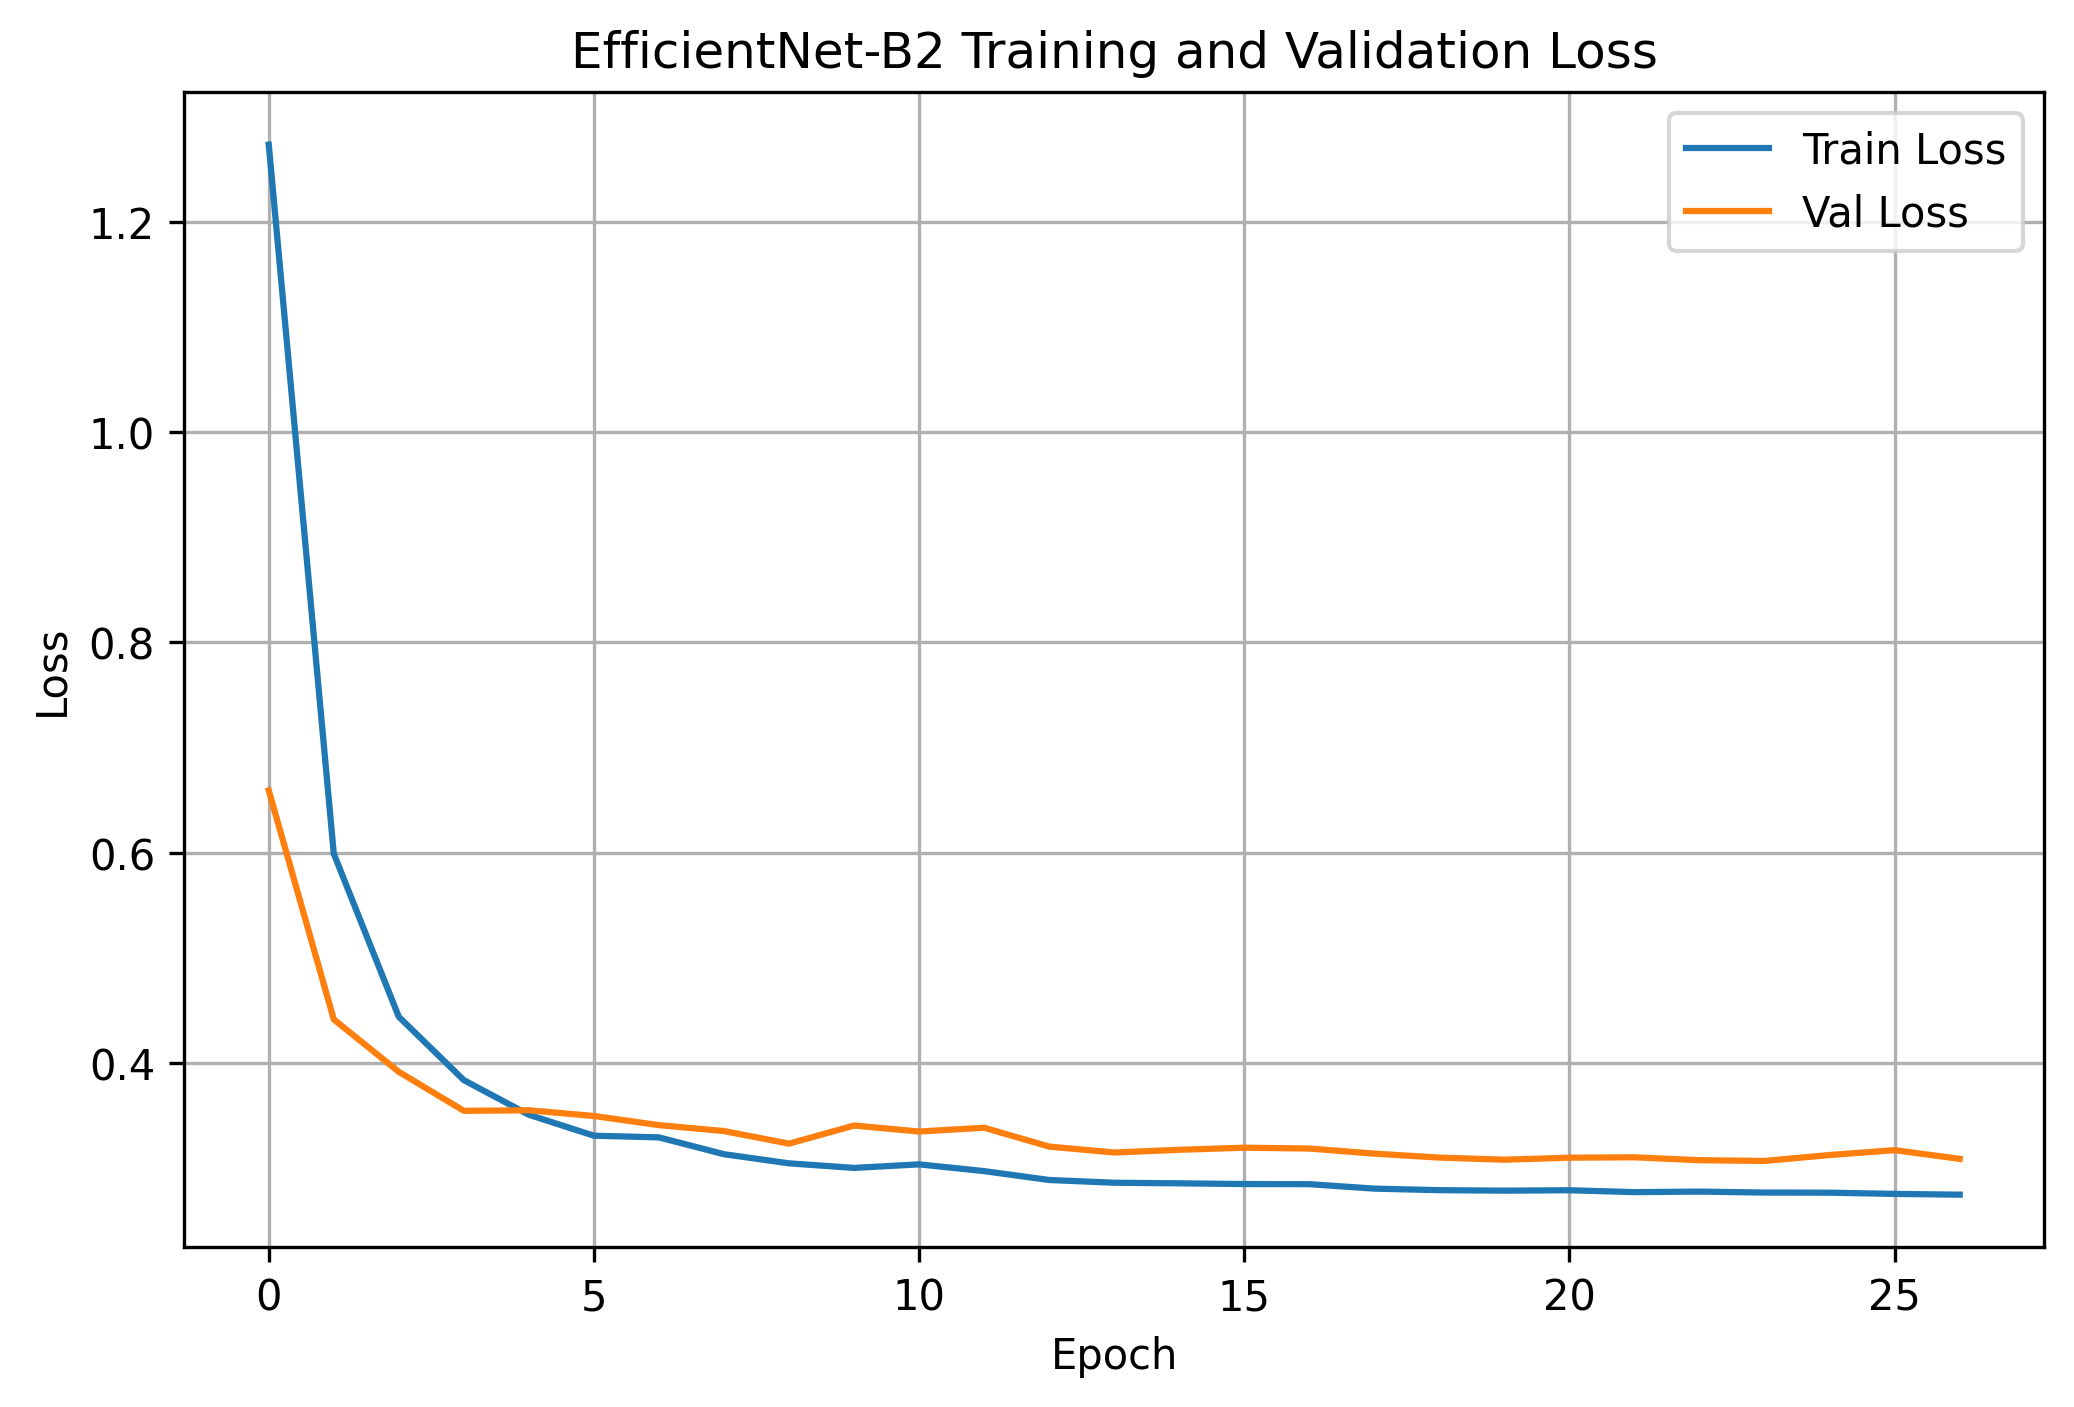
\includegraphics[width=\linewidth]{loss_curve.png}
		\small (a) Loss
	\end{minipage}
	\hfill
	\begin{minipage}{0.32\textwidth}
		\centering
		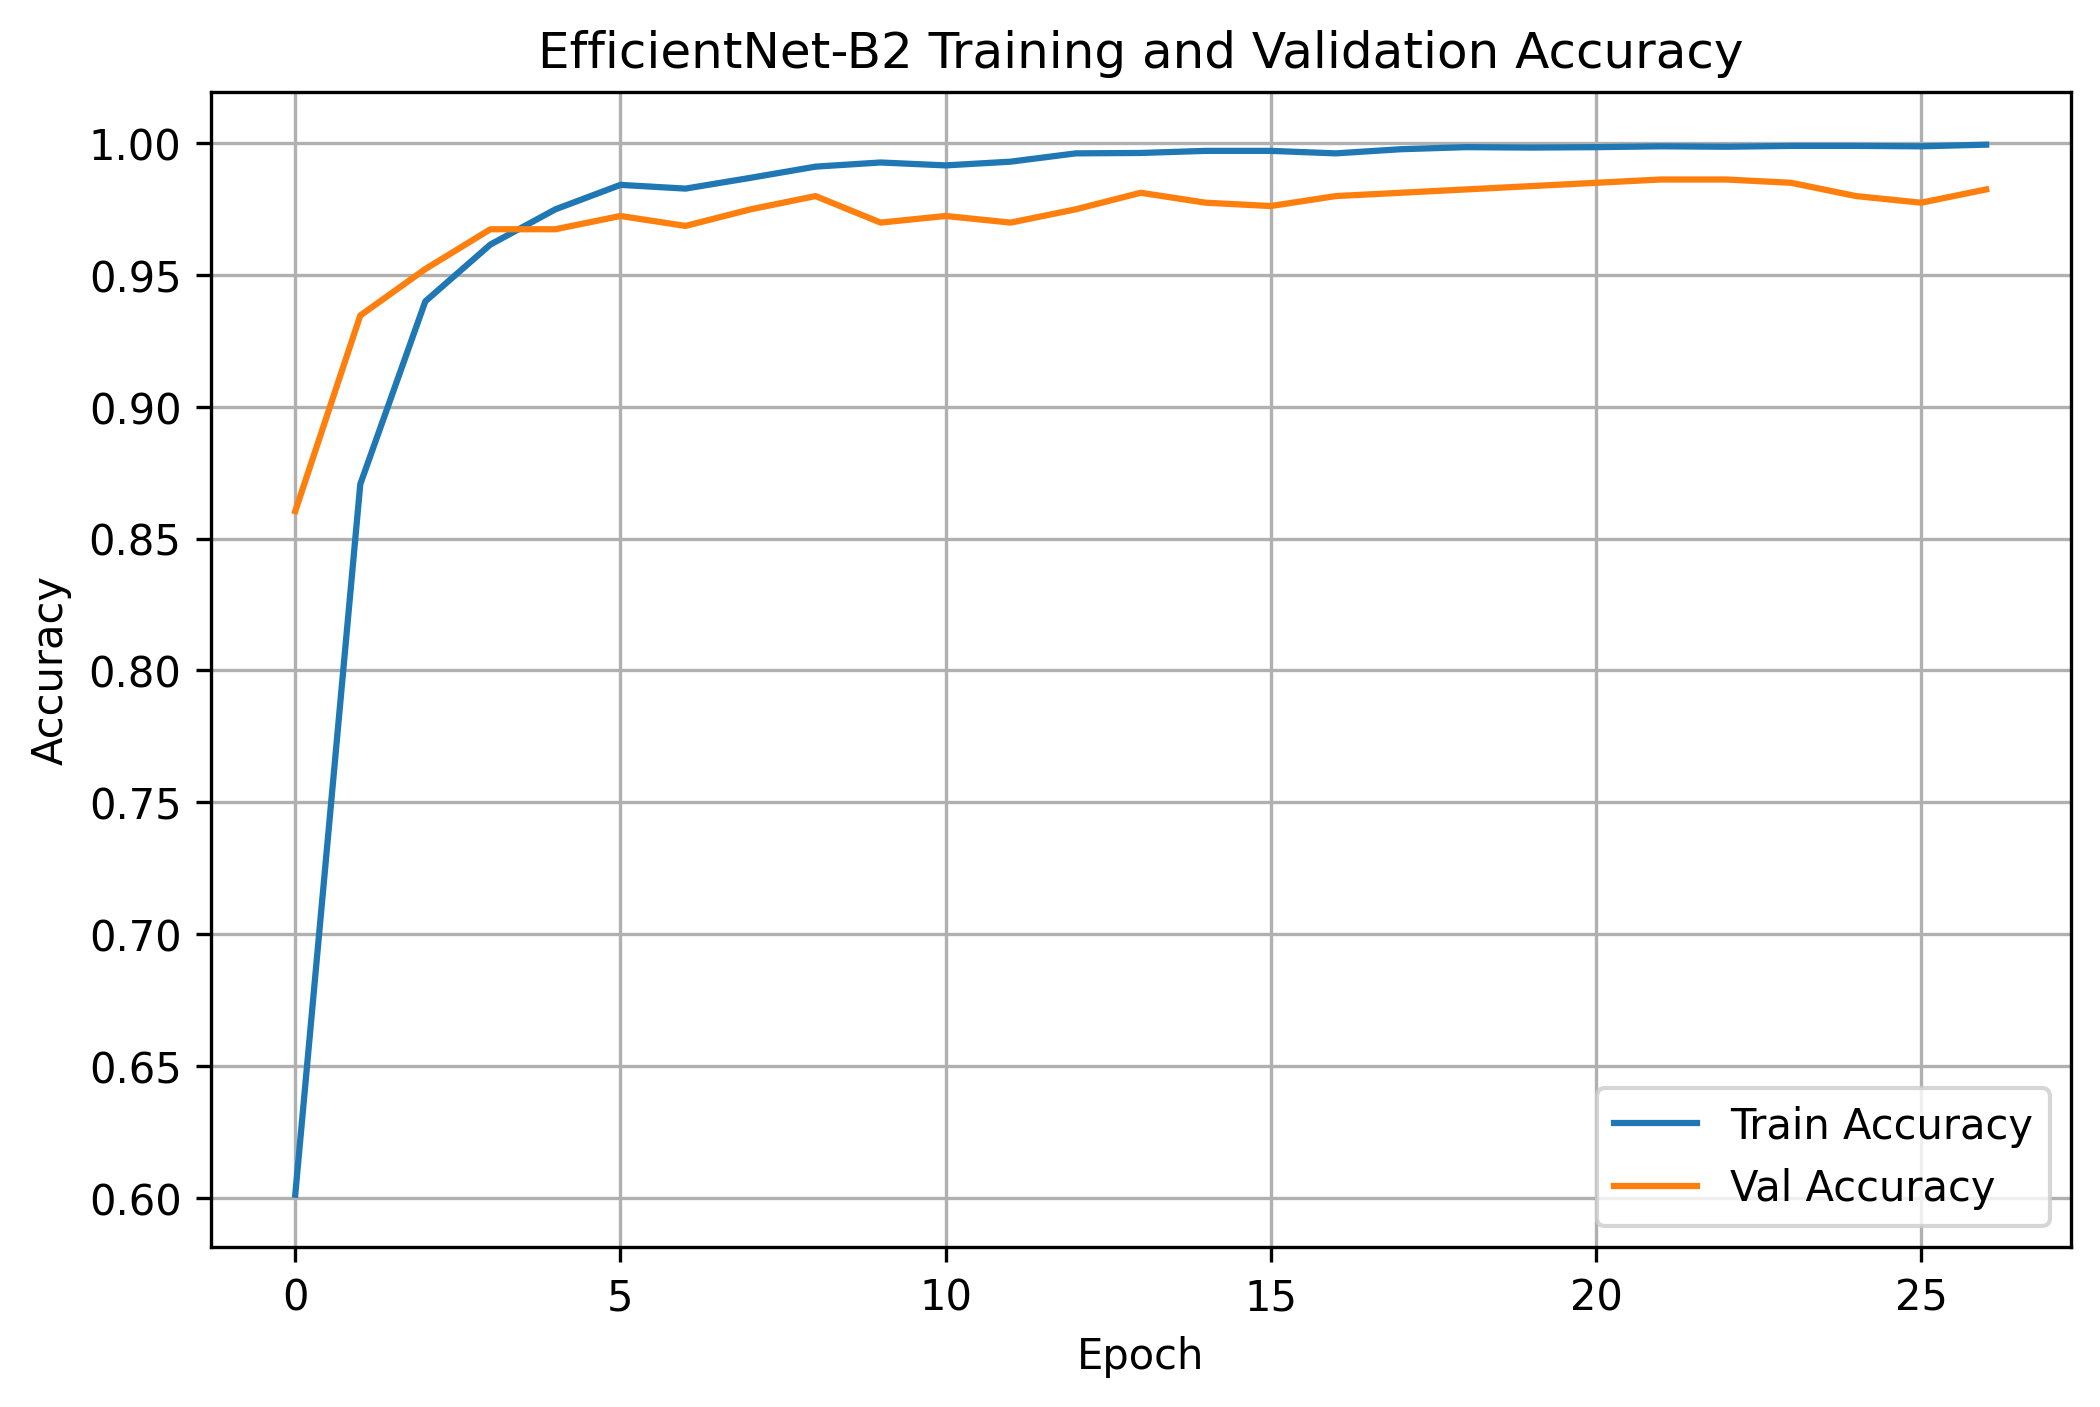
\includegraphics[width=\linewidth]{accuracy_curve.png}
		\small (b) Accuracy
	\end{minipage}
	\hfill
	\begin{minipage}{0.32\textwidth}
		\centering
		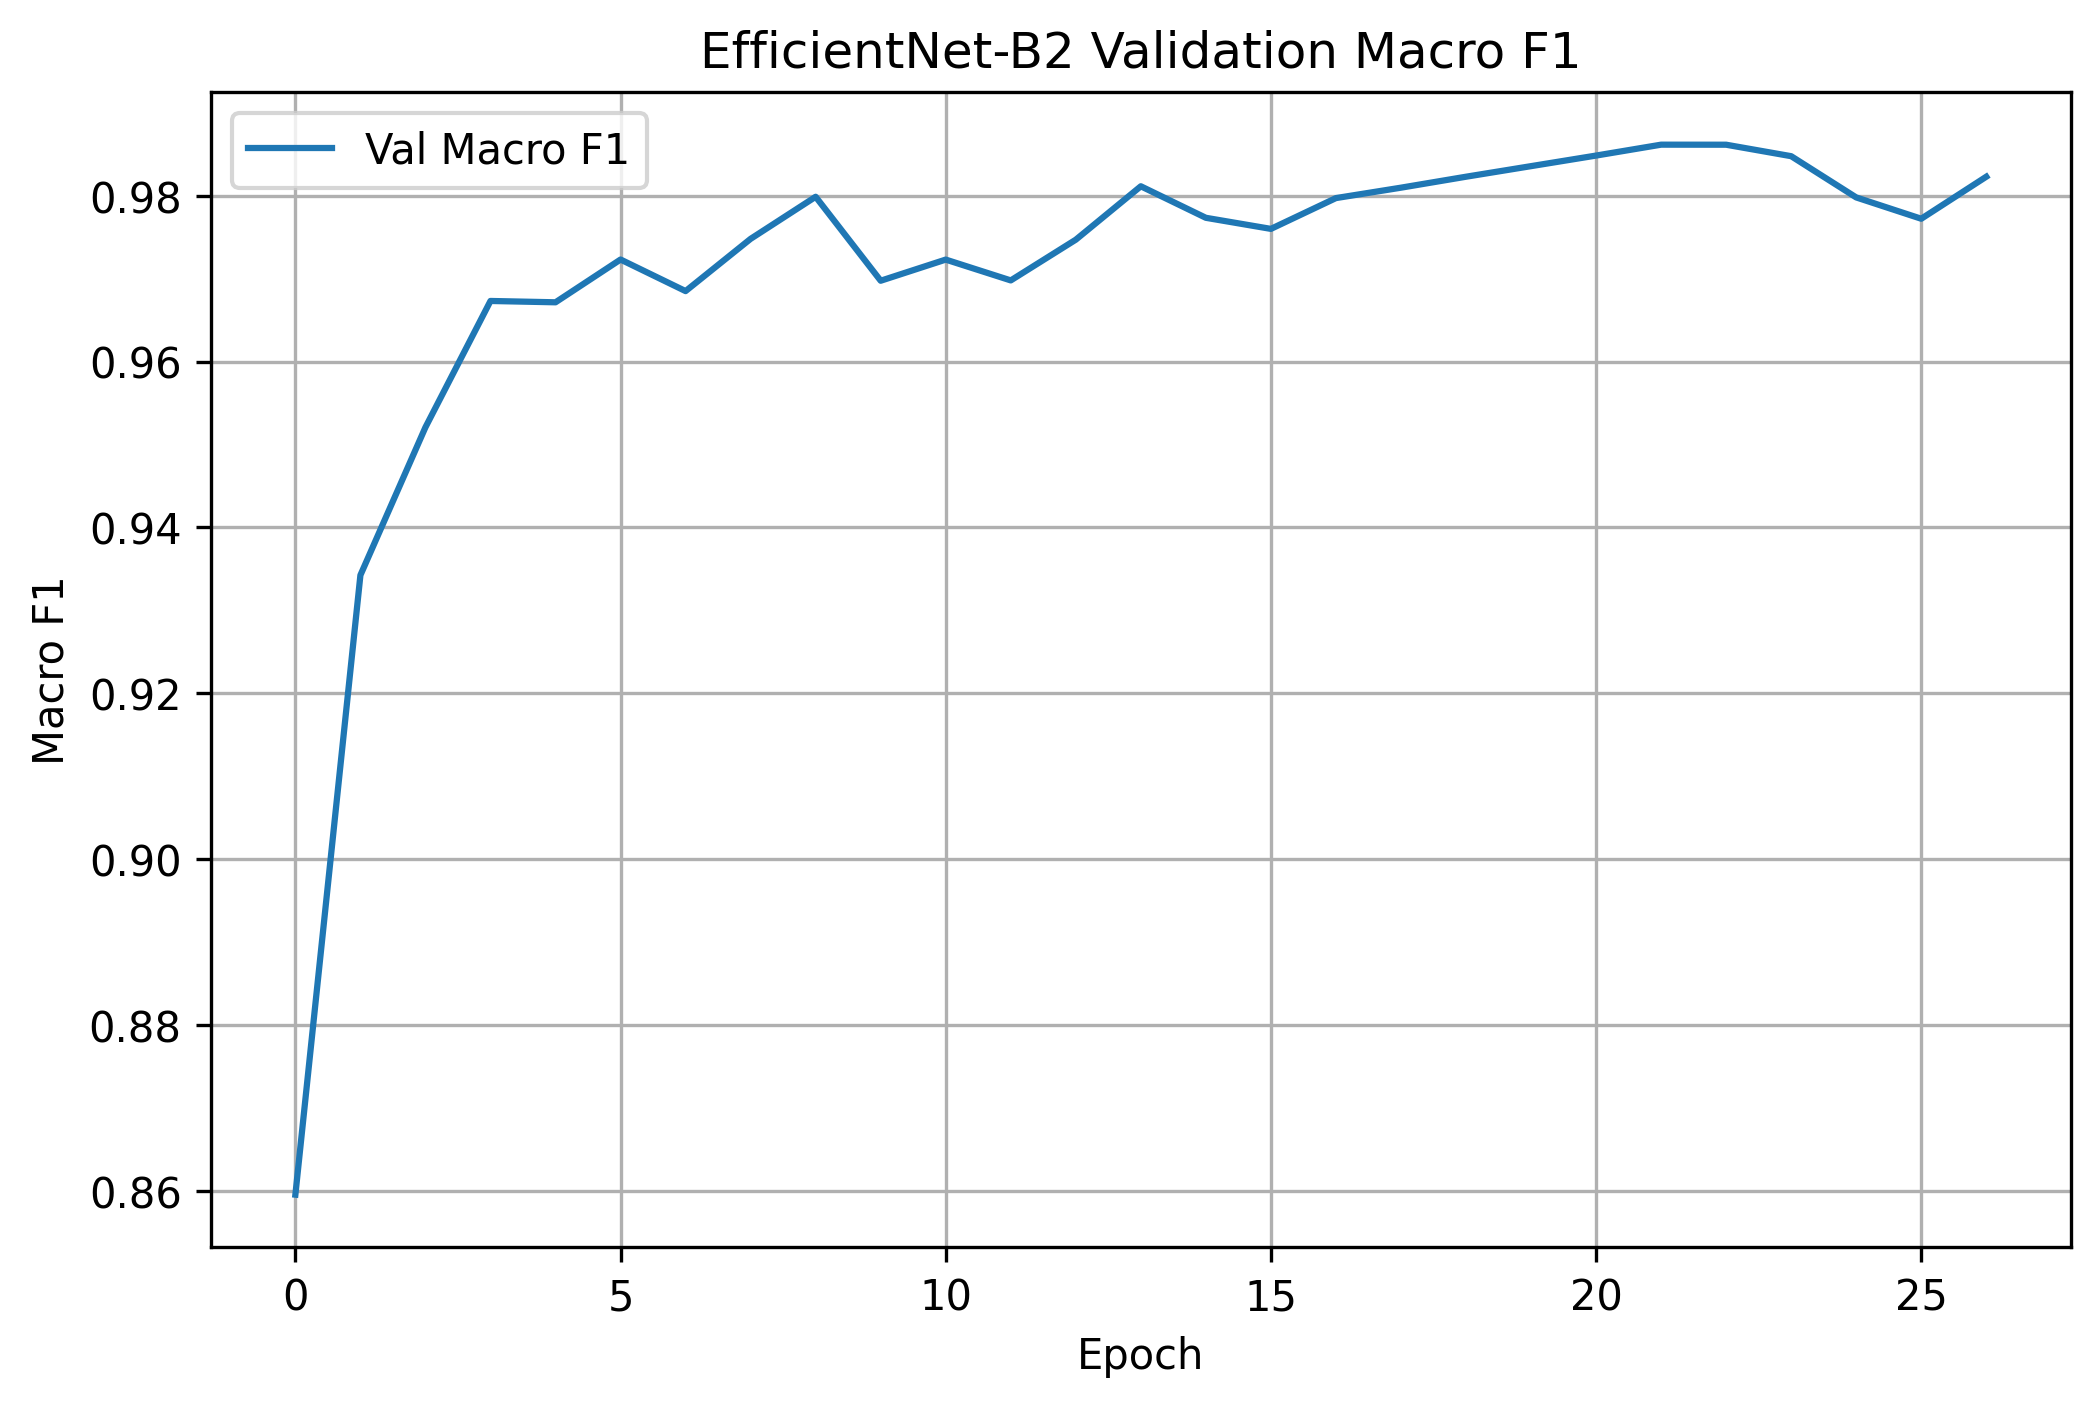
\includegraphics[width=\linewidth]{val_macro_f1_curve.png}
		\small (c) Validation macro F1
	\end{minipage}
	\caption{Eğitim sürecine ait loss, accuracy ve validation macro F1 grafikleri}
	\label{fig:training_curves}
\end{figure*}

\subsection{Test Sonuçları}

Model, ayrılmış test seti üzerinde değerlendirilmiştir. Toplam 796 test
görseli kullanılmıştır. Değerlendirme sonucunda 0.9698 accuracy, 0.9710
macro precision, 0.9699 macro recall ve 0.9700 macro F1 elde edilmiştir.
F1 skorunun proje kapsamında birincil metrik olarak değerlendirildiği
dikkate alındığında, modelin sınıflar arasında dengeli bir performans
sergilediği görülmektedir.

\begin{table}[H]
\centering
\caption{Genel Test Metrikleri}
\label{tab:test_metrics}
\small
\begin{tabular}{|l|r|}
\hline
\textbf{Metrik} & \textbf{Değer} \\
\hline
Accuracy & 0.9698 \\
Macro Precision & 0.9710 \\
Macro Recall & 0.9699 \\
Macro F1 & 0.9700 \\
Weighted Precision & 0.9710 \\
Weighted Recall & 0.9698 \\
Weighted F1 & 0.9699 \\
\hline
\end{tabular}
\end{table}

\begin{table}[H]
\centering
\caption{Sınıf Bazlı Test Sonuçları}
\label{tab:class_metrics}
\scriptsize
\begin{tabular}{|l|r|r|r|r|}
\hline
\textbf{Sınıf} & \textbf{Precision} & \textbf{Recall} & \textbf{F1} & \textbf{Support} \\
\hline
SUV & 0.96 & 0.94 & 0.95 & 100 \\
VAN & 0.99 & 1.00 & 1.00 & 100 \\
STATION\_WAGON & 0.97 & 1.00 & 0.99 & 100 \\
MICRO & 0.99 & 0.98 & 0.98 & 96 \\
OPEN\_WHEEL & 1.00 & 1.00 & 1.00 & 100 \\
SEDAN & 0.99 & 0.90 & 0.94 & 100 \\
HATCHBACK & 0.88 & 0.95 & 0.91 & 100 \\
PICK\_UP & 1.00 & 0.99 & 0.99 & 100 \\
\hline
\end{tabular}
\end{table}

\subsection{Karışıklık Matrisi Analizi}

Normalize edilmiş karışıklık matrisi incelendiğinde VAN ve OPEN\_WHEEL
sınıflarında oldukça yüksek başarı elde edildiği görülmektedir. PICK\_UP
ve MICRO sınıfları da güçlü ayrışmıştır. En belirgin karışmalar ise
SEDAN, HATCHBACK ve STATION\_WAGON sınıfları arasında oluşmuştur. Bu
durum beklenen bir sonuçtur; çünkü bu sınıflar bazı açılardan benzer
tavan çizgisi, arka bagaj yapısı ve gövde oranlarına sahip olabilir.

\begin{figure*}[!t]
	\centering
	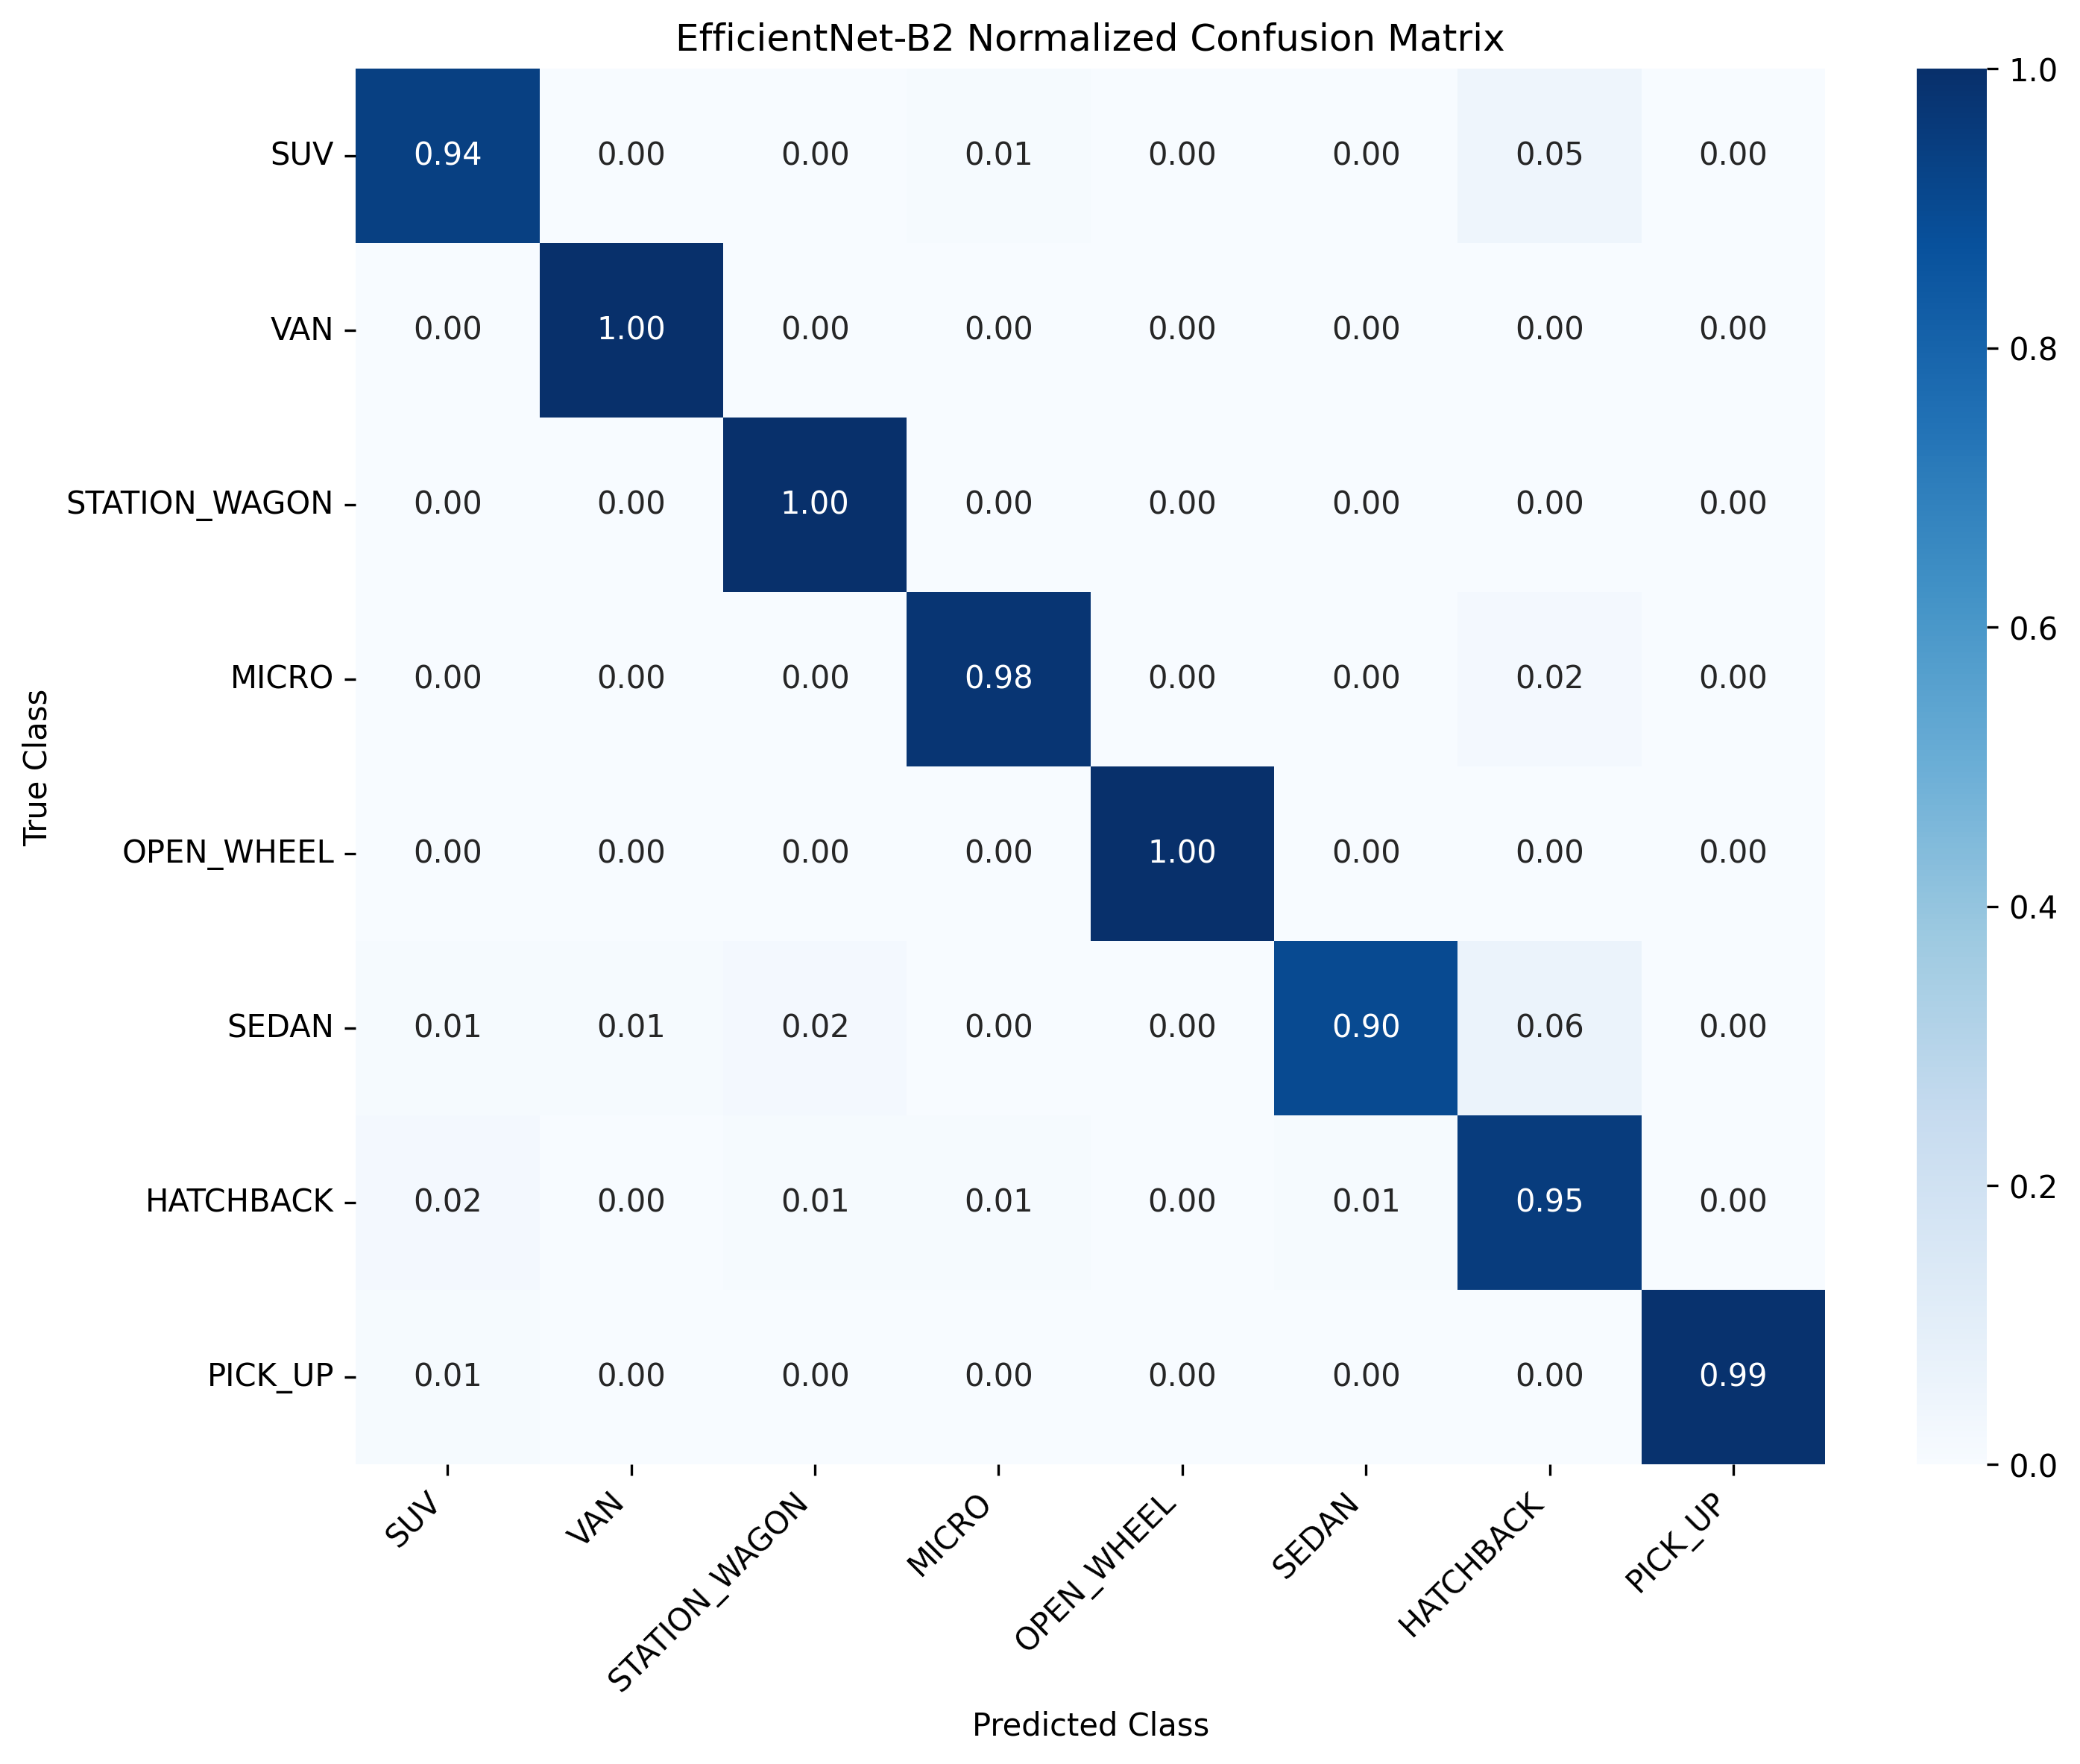
\includegraphics[width=0.88\textwidth]{normalized_confusion_matrix.png}
	\caption{Normalize edilmiş karışıklık matrisi}
	\label{fig:confusion_matrix}
\end{figure*}

\section{WEB ARAYÜZÜ}

Model, Streamlit tabanlı bir web arayüzüne entegre edilmiştir. Arayüzde
kullanıcı bir araç görseli yükleyebilmekte, yüklenen görselin önizlemesini
görebilmekte ve ``Tahmin Yap'' butonu ile model tahminini
çalıştırabilmektedir. Tahmin sonucunda sınıf adı, hocaların kullandığı
1-8 arası sınıf numarası, güven skoru ve tüm sınıflar için olasılık
dağılımı gösterilmektedir.
\vspace{0.4cm}

Arayüzde de B2 V4 model ile aynı preprocessing kullanılmaktadır. Böylece web
arayüzünde alınan tahminler ile test/evaluation scriptlerinde alınan
tahminler arasında preprocessing kaynaklı tutarsızlık oluşması
engellenmiştir. Model tek sefer yüklenmekte ve Streamlit cache mekanizması
ile tekrar tekrar yükleme maliyeti azaltılmaktadır.

\begin{figure}[H]
	\centering
	\includegraphics[width=0.98\columnwidth]{web_interface_main.jpg}
	\caption{Streamlit web arayüzünde görsel yükleme ve tahmin sonucu ekranı}
	\label{fig:web_interface_main}
\end{figure}

\begin{figure}[H]
	\centering
	\includegraphics[width=0.92\columnwidth]{web_interface_probabilities.jpg}
	\caption{Streamlit web arayüzünde sınıf olasılıkları grafiği ve tablo çıktısı}
	\label{fig:web_interface_probabilities}
\end{figure}



\section{TESLİM VE TEST ENTEGRASYONU}

Nihai değerlendirme için ayrı bir teslim klasörü hazırlanmıştır. Bu
klasörde PredictionScript.txt, best\_model.pth ve class\_names.json
dosyaları bulunmaktadır. Model dosyası B2 V4 EfficientNet-B2 modelidir ve
yaklaşık 29.86 MB boyutundadır. Böylece 95 MB sınırının oldukça altında
kalınmıştır.
\vspace{0.4cm}

PredictionScript.txt dosyası Python ile yazılmıştır ve Colab ortamında
çalışacak şekilde hazırlanmıştır. Script içinde \texttt{Predict(file\_path)}
fonksiyonu bulunmaktadır. Bu fonksiyon testdata klasörünü recursive
olarak gezmekte ve her görsel için aşağıdaki formatta tahmin satırı
üretmektedir:

\begin{flushleft}
\ttfamily
filename.jpg | Pred: 1
\end{flushleft}
\normalfont

Hocaların verdiği değerlendirme scriptinde satırlar `` | '' ayracına ve
``:'' karakterine göre okunduğu için bu format birebir korunmuştur.
Ayrıca dosya adı olarak yalnızca \texttt{image\_path.name} kullanılmış,
tam dosya yolu yazılmamıştır. Script çıktı olarak hocanın belirttiği
Preds.txt dosyasını üretmektedir.
\vspace{0.4cm}

Teslim klasöründe model dosyasının yanında \texttt{class\_names.json}
dosyası da bulundurulmuştur. Bu dosya, modelin çıkış indeksleri ile sınıf
adları arasındaki eşleşmeyi korumaktadır. Tahmin sırasında model sıfırdan
başlayan indeks üretmekte, teslim formatında ise sınıflar 1-8 aralığında
numaralandırılmaktadır. Bu nedenle script, model çıktısındaki indeksi
bir artırarak hocanın beklediği sınıf numarasını üretmektedir.
\vspace{0.4cm}

PredictionScript dosyası, değerlendirme ortamında ek bir arayüze ihtiyaç
duymadan çalışacak şekilde hazırlanmıştır. Script, test klasörü içinde alt
klasörler bulunsa bile görselleri recursive olarak okumakta, dosyaları ada
göre sıralamakta ve her tahmin satırını hem ekrana yazdırmakta hem de
\texttt{Preds.txt} dosyasına kaydetmektedir. Böylece aynı model; Streamlit
arayüzünde tek görsel tahmini, toplu test aracı ve otomatik değerlendirme
scripti üzerinden tutarlı biçimde kullanılabilmektedir.

\section{TEKNİK ZORLUKLAR VE DEĞERLENDİRME}

Proje sürecinde en önemli zorluk, sınıflar arasındaki görsel benzerlikler
ve veri seti temizliği olmuştur. SEDAN, HATCHBACK ve STATION\_WAGON
sınıfları bazı açılarda birbirine oldukça benzediği için manuel veri
kontrolü yapılmış ve model bazlı arama sorguları ile daha temiz aday
görseller toplanmıştır. MICRO ve OPEN\_WHEEL sınıfları ise referans veri
setlerinde yeterli düzeyde bulunmadığından bu sınıflar için ayrıca aday
havuzları oluşturulmuştur.
\vspace{0.4cm}

Bir diğer zorluk, modelin Colab ortamında eğitilip yerel proje ve teslim
scriptleriyle uyumlu hale getirilmesidir. Bu nedenle preprocessing
mantığı tüm tahmin dosyalarında aynılaştırılmış, B2 V4 model için
ResizeWithPadding(224) yaklaşımı hem arayüzde hem de PredictionScript
dosyasında kullanılmıştır. Böylece eğitim ve tahmin aşamaları arasındaki
dağılım farkı azaltılmıştır.
\vspace{0.4cm}

Model seçimi aşamasında da yalnızca en yüksek accuracy değerine bakılmamış,
macro F1, dosya boyutu, tahmin hızı ve sınıflar arası dengeli başarı birlikte
değerlendirilmiştir. ResNet18 güçlü bir alternatif üretmiş, EfficientNet-B3
ise daha büyük olmasına rağmen final B2 modelinden daha iyi sonuç
vermemiştir. Bu nedenle EfficientNet-B2, hem doğruluk hem de teslim
kısıtları açısından en dengeli seçenek olarak belirlenmiştir.

\section{SONUÇ}

Bu çalışmada, sekiz sınıflı araba gövde tipi sınıflandırma problemi için
EfficientNet-B2 tabanlı bir derin öğrenme sistemi geliştirilmiştir. Veri
seti farklı kaynaklardan toplanmış, manuel kontrol ile temizlenmiş ve
sınıf dengesi gözetilerek train/validation/test olarak ayrılmıştır. Farklı
model adayları karşılaştırıldıktan sonra EfficientNet-B2, başarı ve model
boyutu arasında en uygun dengeyi sağladığı için final model olarak
seçilmiştir. Model, Google Colab ortamında T4 GPU ile eğitilmiş ve 29.86 MB
boyutunda bir state\_dict dosyası olarak kaydedilmiştir.
\vspace{0.4cm}

Test sonuçları, modelin genel olarak güçlü ve dengeli bir performans
sergilediğini göstermiştir. Macro F1 değerinin 0.9700 olması, sınıflar
arası dengenin korunduğunu göstermektedir. En yüksek başarı VAN,
OPEN\_WHEEL ve PICK\_UP sınıflarında elde edilirken, en fazla karışma
SEDAN, HATCHBACK ve STATION\_WAGON sınıfları arasında gözlenmiştir.
\vspace{0.4cm}

Modelin web arayüzüne entegre edilmesi ve PredictionScript.txt dosyasının
hoca değerlendirme formatına uygun hazırlanması ile proje hem canlı demo
hem de otomatik test senaryosu için çalışabilir hale getirilmiştir. Gelecek
çalışmalarda benzer gövde tipleri arasındaki ayrımı güçlendirmek için daha
fazla gerçek dünya görseli, daha hedefli veri artırma teknikleri ve hata
analizi sonucunda seçilen zor örneklerle ek eğitim yapılabilir.

\section{YAZAR KATKILARI}

Bu proje, iki yazarın ortak çalışması ile geliştirilmiştir. Veri toplama,
manuel veri temizleme, model eğitimi, test analizi, Streamlit arayüzü,
PredictionScript entegrasyonu ve raporlama aşamaları birlikte
yürütülmüştür. Çalışma boyunca kararlar ortaklaşa alınmış ve uygulama ile
dokümantasyon süreçlerinde dengeli sorumluluk paylaşımı sağlanmıştır.

\begin{thebibliography}{12}

\bibitem{efficientnet}
M. Tan and Q. V. Le, ``EfficientNet: Rethinking Model Scaling for Convolutional Neural Networks,'' \emph{International Conference on Machine Learning}, 2019.

\bibitem{pytorch}
PyTorch, \emph{PyTorch Documentation}, [Çevrimici]. Erişim: \url{https://pytorch.org/docs/stable/index.html}

\bibitem{torchvision}
Torchvision, \emph{Torchvision Models Documentation}, [Çevrimici]. Erişim: \url{https://pytorch.org/vision/stable/models.html}

\bibitem{streamlit}
Streamlit, \emph{Streamlit Documentation}, [Çevrimici]. Erişim: \url{https://docs.streamlit.io/}

\bibitem{sklearn}
Scikit-learn, \emph{Model Evaluation Documentation}, [Çevrimici]. Erişim: \url{https://scikit-learn.org/stable/modules/model_evaluation.html}

\bibitem{carscropped}
A. Boukhris, \emph{Cars Body Type Cropped}, Kaggle Dataset, [Çevrimici]. Erişim: \url{https://www.kaggle.com/datasets/ademboukhris/cars-body-type-cropped}

\bibitem{stanfordcars}
M. Mahurkar, \emph{Stanford Car Body Type Data}, Kaggle Dataset, [Çevrimici]. Erişim: \url{https://www.kaggle.com/datasets/mayurmahurkar/stanford-car-body-type-data}

\bibitem{imagenet}
J. Deng et al., ``ImageNet: A Large-Scale Hierarchical Image Database,'' \emph{IEEE Conference on Computer Vision and Pattern Recognition}, 2009.

\bibitem{pillow}
Pillow, \emph{Pillow Documentation}, [Çevrimici]. Erişim: \url{https://pillow.readthedocs.io/}

\end{thebibliography}

\end{document}
